In order to generate the key that will be sent to Bob, Alice creates a random string of $2n$
qubits encoded in polarized photons and emits them. She chooses a specific polarization for
each photon among four possibilities, two pairs of which are associated with two
different linear polarization bases: \{$|0\rangle$, $|1\rangle$\} (or\ `$\bm{+}$') and \{$|+\rangle$, $|-\rangle$\} 
(or\ `$\bm{\times}$').
Two can be described as being along the $x$, $y$ axes, often denoted as $\bm{\uparrow}$ (Vertical)
and $\bm{\rightarrow}$ (Horizontal), while the other two polarizations are at a $+\ang{45}$ orientation 
from the $x$ and $y$ axes and are usually denoted as $\bm{\nwarrow}$ (Left) and $\bm{\nearrow}$ (Right).
Each pair corresponds to two orthogonal ($\ang{90}$ difference) polarizations. Furthermore, the two pairs
correspond to two separate polarizing beam splitter orientations, $\ang{45}$ from each other.
\begin{center}
    \begin{tabular}{|p{4.7cm}|p{4.7cm}|}
    \hline
        \hfil$|{\bm{\rightarrow}}\rangle = |0\rangle$ & 
        \hfil$|{\bm{\uparrow}}\rangle = |1\rangle$ \\
    \hline
         $|{\bm{\nwarrow}}\rangle = \dfrac{(|{\bm{\rightarrow}}\rangle + |{\bm{\uparrow}}\rangle)}{\sqrt{2}} = |+\rangle$ &
         $|{\bm{\nearrow}}\rangle = \dfrac{(|{\bm{\rightarrow}}\rangle - |{\bm{\uparrow}}\rangle)}{\sqrt{2}} = |-\rangle$ \\
    \hline
  \end{tabular}
\end{center}
When Bob receives a photon, he realizes its polarization with a polarization beam splitter
placed at a random orientation: either the vertical $\{\bm{\uparrow} , \bm{\rightarrow}\}$ or
the $45^o$ $\{\bm{\nwarrow} , \bm{\nearrow}\}$.
If his choice corresponds to the polarization used by Alice during transmission, he obtains the result
corresponding to the value chosen and sent by Alice. 
E.g. If Alice sends a photon with a $\{\bm{\uparrow} ,\bm{\rightarrow}\}$
polarization and Bob places his beam splitter at the $\ang{45}$ $\{\bm{\nwarrow} , \bm{\nearrow}\}$ orientation, then he will
obtain a random result, uncorrelated to Alice's initial choice.
So, retrieving the corrent data bits that were sent by Alice depends 
on his choosing as a measuring basis one that corresponds to the polarization basis chosen by Alice.
But, how will Bob know which qubits he received are the correct ones? The answer is twofold.
The first process is called {\it reconciliation} or {\it sifting}: In order for Alice and Bob to agree
upon the congruent data bits, they must first compare their bases and keep only the bits
corresponding to their specific matching bases. It suffices for Bob to announce his chosen bases on the
public channel and for Alice to reply with the ones that were correct (same as her polarization bases), 
prompting Bob to discard bits corresponding to the rest (non-corresponding bases). 
Ideally, if there was no eavesdropping, both are left with an identical key (see Fig. \ref{fig4}). 
Realistically, Bob is left with a key composed of bits measured using identical bases. 
That key will then have to pass through the second process, {\it error correction}. 
In both cases, the resulting key, produced by discarding the bits where Alice 
and Bob’s bases differ, is called the {\it sifted key}.
\begin{figure}[!h]
\centerline{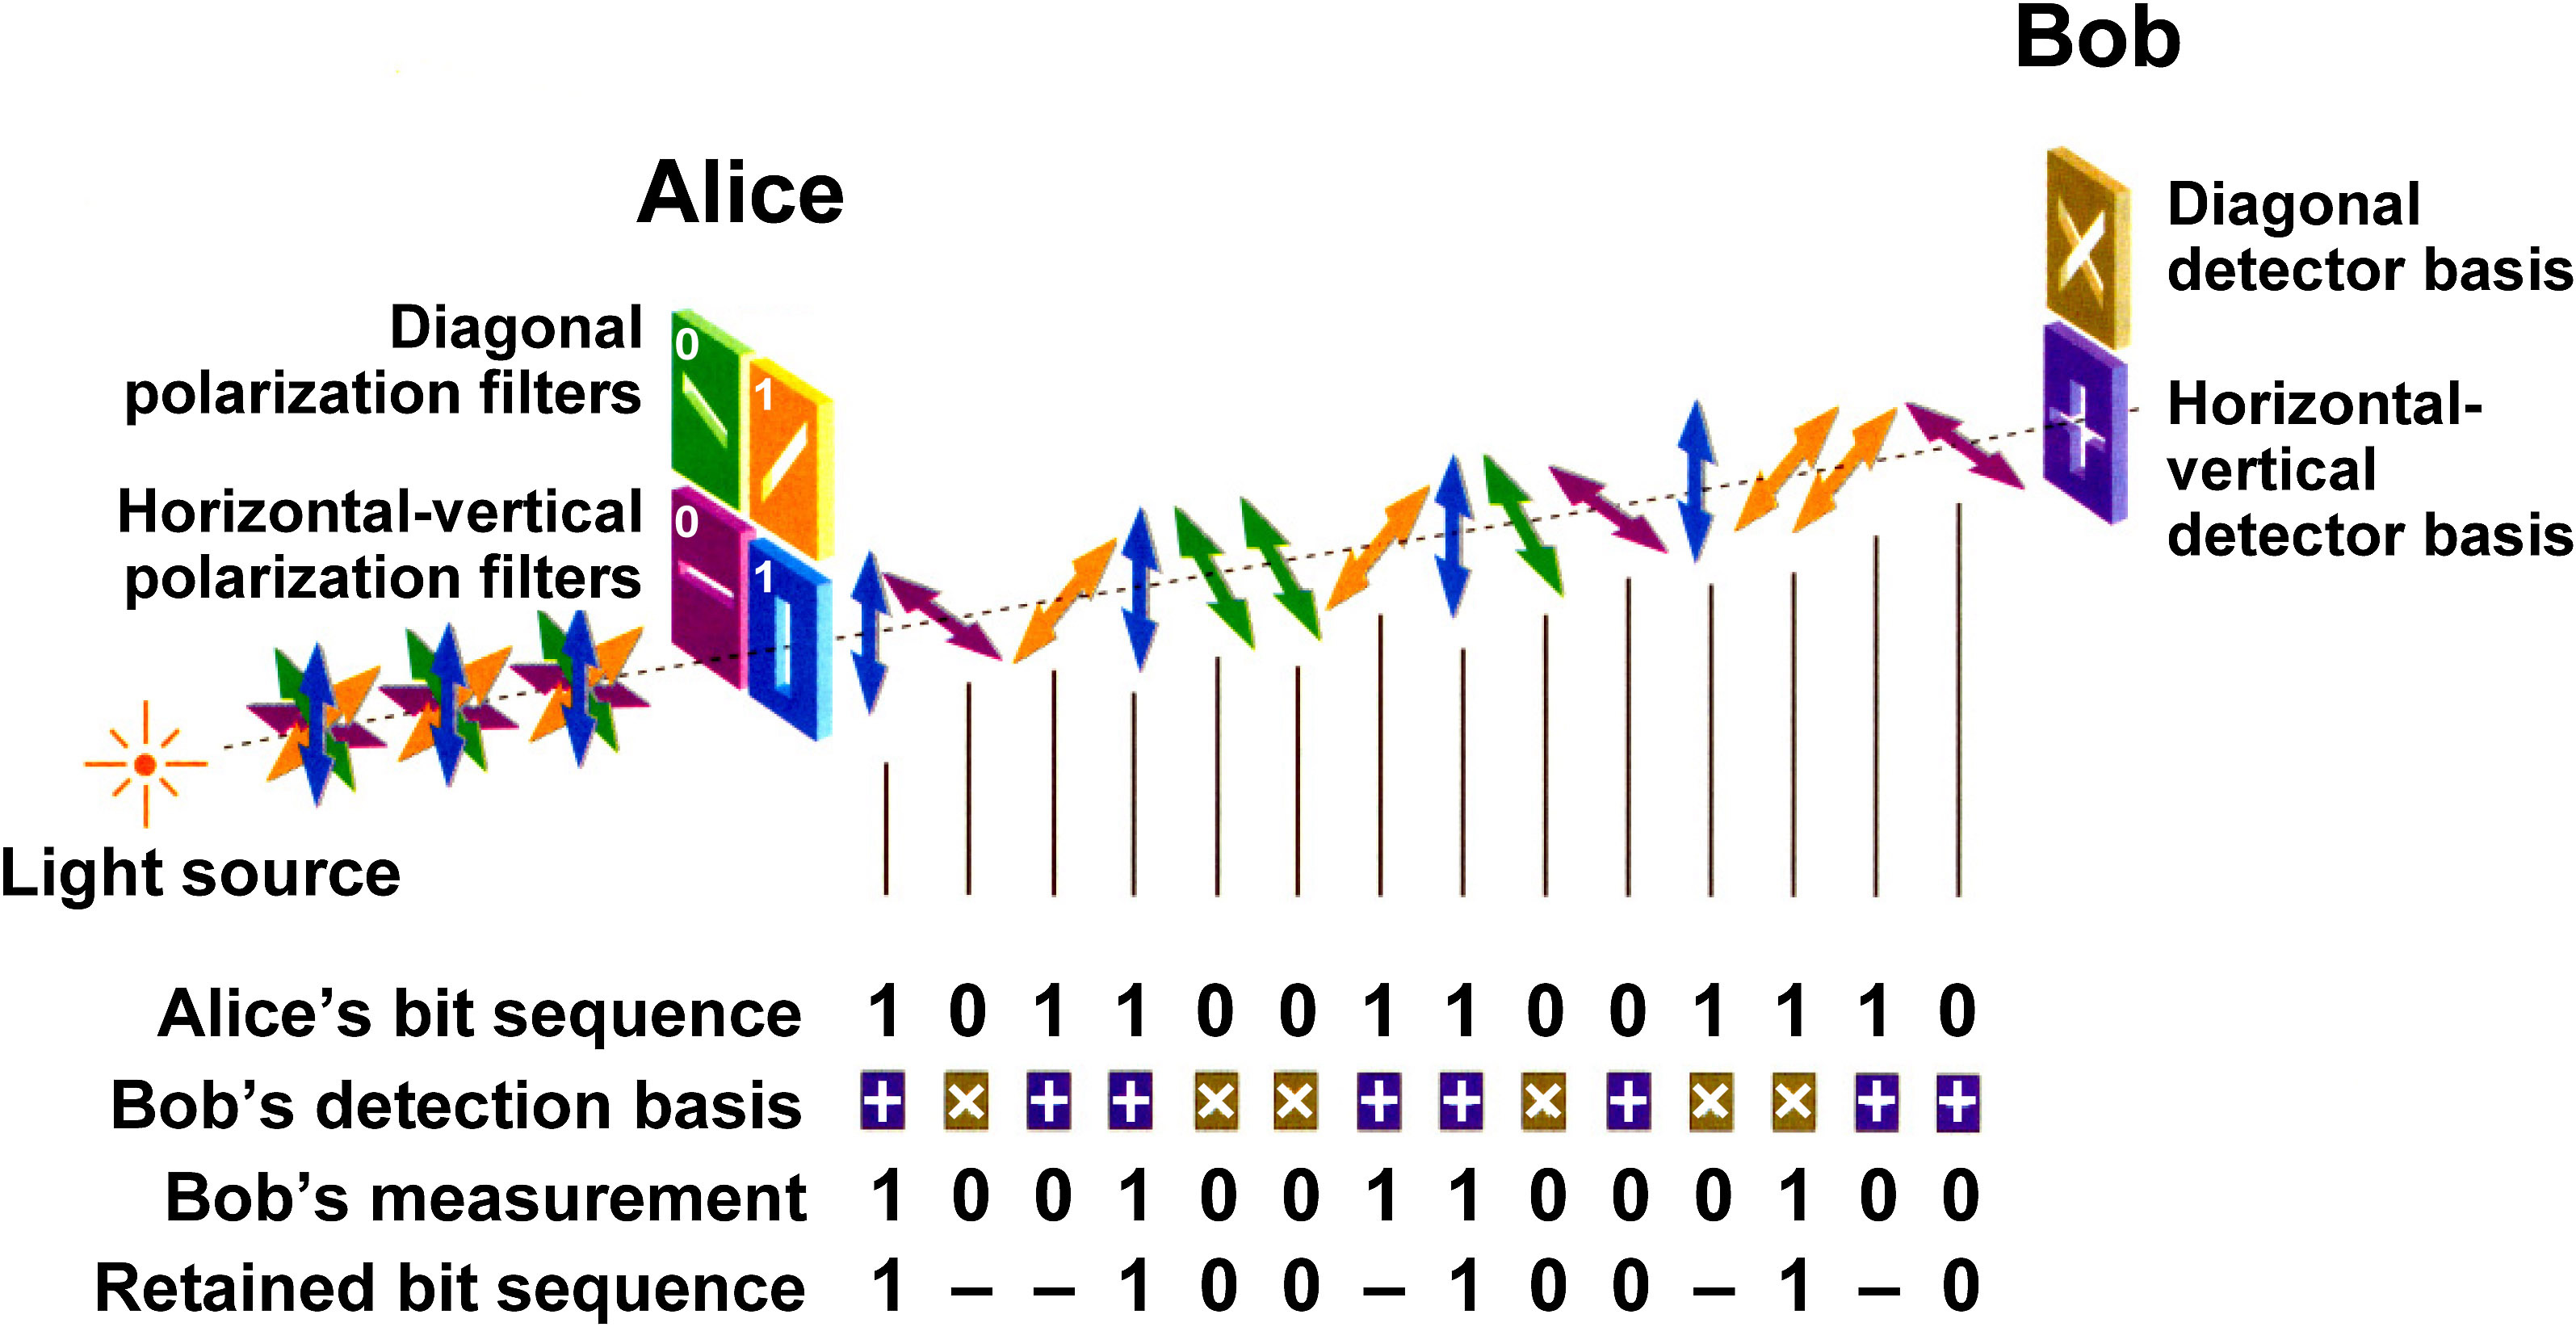
\includegraphics[width=\textwidth,height=\textheight,keepaspectratio]{4.png}}
\caption{An ideal QKD, with no Eve}
\label{fig4}
\end{figure}

It shall be seen that if specific communicated and compared qubits of Bob's {\it sifted key}
differ despite their bases being identical, it will mean that someone has been eavesdropping.

